\documentclass[11pt]{article}

% Change "review" to "final" to generate the final (sometimes called camera-ready) version.
% Change to "preprint" to generate a non-anonymous version with page numbers.
\usepackage[review]{acl}
\usepackage{booktabs} 
\usepackage{minted}
\usepackage{float}
% Standard package includes
\usepackage{times}
\usepackage{latexsym}
\usepackage{listings}
\usepackage{enumitem}
\setlist[itemize]{itemsep=1pt, topsep=3pt}

% Modern code style with clean aesthetics
\definecolor{codebg}{RGB}{248,248,248}
\definecolor{codegreen}{RGB}{40,160,80}
\definecolor{codeblue}{RGB}{50,90,180}
\definecolor{codeorange}{RGB}{220,100,0}
\definecolor{codegray}{RGB}{100,100,100}

\lstdefinestyle{pythonstyle}{
    backgroundcolor=\color{codebg},
    commentstyle=\color{codegreen}\itshape,
    keywordstyle=\color{codeblue}\bfseries,
    numberstyle=\tiny\color{codegray},
    stringstyle=\color{codeorange},
    basicstyle=\ttfamily\small,
    breaklines=true,
    breakatwhitespace=true,
    frame=l,
    framerule=2pt,
    rulecolor=\color{codeblue!60},
    xleftmargin=8pt,
    captionpos=b,
    language=Python,
    showstringspaces=false,
    tabsize=4,
    morekeywords={dataclass,Enum,Optional,List,Tuple,Dict,field}
}

\lstset{style=pythonstyle}

% For proper rendering and hyphenation of words containing Latin characters (including in bib files)
\usepackage[T1]{fontenc}
\usepackage{amsmath}
\usepackage{amssymb} 

% For Vietnamese characters
% \usepackage[T5]{fontenc}
% See https://www.latex-project.org/help/documentation/encguide.pdf for other character sets

% This assumes your files are encoded as UTF8
\usepackage[utf8]{inputenc}

% This is not strictly necessary, and may be commented out,
% but it will improve the layout of the manuscript,
% and will typically save some space.
\usepackage{microtype}

% This is also not strictly necessary, and may be commented out.
% However, it will improve the aesthetics of text in
% the typewriter font.
\usepackage{inconsolata}

%Including images in your LaTeX document requires adding
%additional package(s)
\usepackage{graphicx}
\usepackage{pgfplots}
\usepackage{tikz}
\pgfplotsset{compat=1.17}
\usetikzlibrary{patterns}

% If the title and author information does not fit in the area allocated, uncomment the following
%
%\setlength\titlebox{<dim>}
%
% and set <dim> to something 5cm or larger.

\makeatletter
\renewcommand\cite{\citep}
\makeatother
\title{Fine-tuning Small LLMs with Graph-Modeled Schemas for Multi-table NL2SQL}

% Author information can be set in various styles:
% For several authors from the same institution:
% \author{Author 1 \and ... \and Author n \\
%         Address line \\ ... \\ Address line}
% if the names do not fit well on one line use
%         Author 1 \\ {\bf Author 2} \\ ... \\ {\bf Author n} \\
% For authors from different institutions:
% \author{Author 1 \\ Address line \\  ... \\ Address line
%         \And  ... \And
%         Author n \\ Address line \\ ... \\ Address line}
% To start a separate ``row'' of authors use \AND, as in
% \author{Author 1 \\ Address line \\  ... \\ Address line
%         \AND
%         Author 2 \\ Address line \\ ... \\ Address line \And
%         Author 3 \\ Address line \\ ... \\ Address line}

\author{Zhanhao Liu \\
  University of Michigan \\
  Ann Arbor, MI \\
  \texttt{zhanhaol@umich.edu} \\\And
  Qiulin Fan \\
  University of Michigan \\
  Ann Arbor, MI \\
  \texttt{
rynnefan@umich.edu} \\}

%\author{
%  \textbf{First Author\textsuperscript{1}},
%  \textbf{Second Author\textsuperscript{1,2}},
%  \textbf{Third T. Author\textsuperscript{1}},
%  \textbf{Fourth Author\textsuperscript{1}},
%\\
%  \textbf{Fifth Author\textsuperscript{1,2}},
%  \textbf{Sixth Author\textsuperscript{1}},
%  \textbf{Seventh Author\textsuperscript{1}},
%  \textbf{Eighth Author \textsuperscript{1,2,3,4}},
%\\
%  \textbf{Ninth Author\textsuperscript{1}},
%  \textbf{Tenth Author\textsuperscript{1}},
%  \textbf{Eleventh E. Author\textsuperscript{1,2,3,4,5}},
%  \textbf{Twelfth Author\textsuperscript{1}},
%\\
%  \textbf{Thirteenth Author\textsuperscript{3}},
%  \textbf{Fourteenth F. Author\textsuperscript{2,4}},
%  \textbf{Fifteenth Author\textsuperscript{1}},
%  \textbf{Sixteenth Author\textsuperscript{1}},
%\\
%  \textbf{Seventeenth S. Author\textsuperscript{4,5}},
%  \textbf{Eighteenth Author\textsuperscript{3,4}},
%  \textbf{Nineteenth N. Author\textsuperscript{2,5}},
%  \textbf{Twentieth Author\textsuperscript{1}}
%\\
%\\
%  \textsuperscript{1}Affiliation 1,
%  \textsuperscript{2}Affiliation 2,
%  \textsuperscript{3}Affiliation 3,
%  \textsuperscript{4}Affiliation 4,
%  \textsuperscript{5}Affiliation 5
%\\
%  \small{
%    \textbf{Correspondence:} \href{mailto:email@domain}{email@domain}
%  }
%}

\begin{document}
\maketitle

\begin{abstract}
Natural Language to SQL (NL2SQL) enables users to query databases using natural language, but multi-table queries involving JOINs and nested subqueries remain challenging. While large language models (LLMs) have shown strong performance, their computational cost limits practical deployment. In this work, we explore parameter-efficient fine-tuning of a 7B-parameter LLM (Qwen-2.5-7B) for complex NL2SQL tasks. Our approach combines three key techniques: (1) graph-based schema representations that explicitly model table relationships and foreign keys, (2) schema linking that maps question words to relevant schema elements, and (3) LoRA fine-tuning with curriculum learning from simple to complex queries. On the Spider benchmark, our method achieves \textbf{41.5\% Exact Match} and \textbf{58.3\% Execution Match} accuracy on 1,034 test queries, significantly outperforming early neural methods (Seq2SQL, SQLNet, SyntaxSQLNet) and achieving competitive performance with specialized graph-based models like IRNet and RAT-SQL. The 16.8\% gap between Exact Match and Execution Match demonstrates that our model generates semantically correct SQL even when syntactically different from gold references. Our results indicate that schema-aware fine-tuning of small LLMs provides a practical and cost-effective approach to NL2SQL, with particular strength on execution-based evaluation. Code is available at \url{https://github.com/qiulinfan/graphNL2SQL}.
\end{abstract}

\section{Introduction}

\subsection{Background and Motivation}
Natural Language to SQL (NL2SQL) enables non-technical users to query relational databases using natural language, bridging the gap between human intent and structured database queries. Early research before the LLM era relied on task-specific encoder--decoder architectures such as Seq2SQL~\cite{Seq2SQL2017}, SQLNet~\cite{SQLnet2017}, SyntaxSQLNet~\cite{SyntaxSQLNet2018}, IRNet~\cite{IRNet2019}, and RAT-SQL~\cite{RatSQL2021}. While these models achieved remarkable progress, they remain fundamentally limited:
\begin{itemize}
    \item They lack general language understanding and exhibit poor few-shot generalization to unseen databases.
    \item Complex queries involving multi-table JOINs and nested subqueries remain challenging.
    \item Models are often tightly coupled to specific benchmarks and do not transfer well.
\end{itemize} 

With the emergence of large language models (LLMs), NL2SQL has become more feasible. General-purpose models like GPT-4 demonstrate strong natural language to code reasoning through in-context learning. However, this shift exposes practical limitations: (1) state-of-the-art methods largely depend on closed-source LLMs with expensive API costs~\cite{LearNAT2025}, and (2) large LLMs (70B+ parameters) are impractical for domain-specific fine-tuning due to massive computational requirements.

\textbf{Our Contribution:} We explore how a \textbf{small-parameter LLM (7B)} can be fine-tuned to achieve strong NL2SQL performance on complex multi-table queries with a fraction of the computational cost. Our approach combines:
\begin{enumerate}
    \item \textbf{Graph-based schema modeling}: Explicitly representing table relationships and foreign keys to strengthen structural reasoning
    \item \textbf{Schema linking}: Mapping question words to relevant schema elements to ground natural language in database structure
    \item \textbf{Parameter-efficient fine-tuning}: Using LoRA with 4-bit quantization to train on consumer hardware
\end{enumerate}

On the Spider benchmark, our fine-tuned Qwen-7B achieves \textbf{41.5\% Exact Match} and \textbf{58.3\% Execution Match}, significantly outperforming early neural methods and achieving competitive results with specialized graph-based models. Notably, our Execution Match exceeds RAT-SQL by 6.0\%, demonstrating that LLM-based approaches generate semantically correct SQL even when syntactically different from gold references.


% \begin{figure*}[t]
%     \centering
%     \includegraphics[width=\textwidth]{image/bird.png}
%     \caption{An example text-to-SQL task from the BIRD dataset. The query involves multiple tables, each with columns containing realistic values (not fully shown here).}
%     \label{fig:bird}
% \end{figure*}

\subsection{Task Definition}

The specific NLP task this project will address is multi-table Natural Language to SQL (NL2SQL) generation. The task of multi-table NL2SQL generation is to take a natural language query as input and automatically produce a syntactically correct and semantically accurate SQL query that retrieves the correct result from a relational database containing multiple interconnected tables. 
\begin{itemize}
    \item Input: a pair of $(\text{SQL schema}, \text{NL query})$. The schema may contain multiple tables with foreign key relationships. (Note: A foreign key is a column, or set of columns, in one table that refers to the primary key of another table.)
    \item Output: a structured SQL query that can be executed on the target database to return the intended result.
\end{itemize}

% \textbf{Current Idea}:

% Our current approach begins with generating a graph representation of the database. This graph is provided to the model alongside the database schema and the natural language (NL) query, both during training and inference.

% To construct the complete graph, we first construct a graph for each table in the database individually, and then connect these graphs by adding edges between tables. The connections will be established either through explicit foreign key relationships provided in the schema or through semantic understanding of column names (e.g., “Birthday” in one table likely corresponds to “DOB” in another). The graphs for individual tables will remain relatively sparse. To illustrate this approach, we will provide an example of our intended graph structure.
% \begin{center}
%     \includegraphics[width=0.5\textwidth]{image/graph.png}
% \end{center}

% Now the graph captures richer representations of the relationships between tables.  We will incorporate this graph representation alongside the original inputs (schema and query) to further train the NL2SQL model using reinforcement learning.
% The training process will leverage three types of feedback: (1) compilability, measuring whether the generated SQL can be executed successfully on the database, (2) accuracy, assessing whether the query retrieves the correct results, and (3) optimization with respect to time and space complexity. 

% Our proposed idea is based on the assumption that incorporating graph representations during training will help the model better capture relationships between tables, thereby enabling it to generate more accurate and reasonable SQL queries that perform "join" between tables.

\section{Data}
\subsection{WikiSQL Dataset}

The \textbf{WikiSQL} dataset~\cite{Seq2SQL2017}, released by Salesforce, is one of the earliest and most widely used benchmarks for NL2SQL models. It contains 15{,}878 natural language (NL) to SQL pairs along with 4{,}550 data tables on which queries can be executed. 

Using this dataset, we evaluated our generated SQL queries in two ways: 1.by directly comparing the predicted SQL with the gold (reference) SQL.2. by executing both queries on the actual table using DuckDB and comparing their outputs.

However, the WikiSQL dataset focuses solely on generating SQL queries over a single table. It does not include joins or nested queries, making it relatively simple. Since our project aims to improve models’ ability to generate SQL across multiple tables and databases, which is a key limitation of many current NL2SQL systems. We also incorporated the Spider dataset for a more realistic and challenging evaluation.
\begin{center}
\fbox{
\parbox{0.95\linewidth}{
\textbf{Examples from the WikiSQL Dataset} \\[0.5em]

\textbf{Example 1} \\
\textbf{Question:} What institution had 6 wins and a current streak of 2? \\
\textbf{GOLD SQL:} \texttt{SELECT "Institution" FROM "table" WHERE "Wins" = 6 AND "Current Streak" = '2'} \\[1em]

\textbf{Example 2} \\
\textbf{Question:} Capital of Brześć nad Bugiem has what population (1931) in 1,000s? \\
\textbf{GOLD SQL:} \texttt{SELECT "Population (1931) in 1,000s" FROM "table" WHERE "Capital" = 'Brześć nad Bugiem'}
}
}
\end{center}
\begin{table*}[htbp]
\centering
\caption{Truncated table for Example 1 from Wikisql dataset (partial columns shown)}
\begin{tabular}{lcccc}
\hline
\textbf{Institution} & \textbf{Wins} & \textbf{Losses} & \textbf{Home Wins} & \textbf{Home Losses} \\
\hline
Boston College Eagles & 6 & 1 & 3 & 1 \\
Clemson Tigers & 9 & 5 & 4 & 3 \\
Duke Blue Devils & 12 & 2 & 5 & 0 \\
Florida State Seminoles & 6 & 8 & 4 & 3 \\
Georgia Tech Yellow Jackets & 4 & 9 & 3 & 2 \\
Maryland Terrapins & 10 & 4 & 5 & 1 \\
... & ... & ... & ... & ... \\
\hline
\end{tabular}
\label{tab:wikisql}
\end{table*}




\subsection{Spider Dataset}

The \textbf{Spider} dataset~\cite{Spider2018}, created by Yale University, covers a wide range of domains and includes many complex SQL queries involving multi-table joins and nested structures. Its development set contains 1{,}034 questions and gold SQL queries across 20 databases, each provided with full schema information.

Compared to WikiSQL, Spider introduces substantially higher difficulty, as queries often involve multiple tables, foreign key reasoning, and advanced SQL operators such as GROUP BY, ORDER BY, and nested subqueries. This makes Spider a more realistic benchmark for assessing compositional generalization and schema understanding.

We preprocess each database schema into a textual graph representation, concatenating table and column names along with their foreign key relationships. This structured representation is provided to the model alongside natural language questions during both training and inference.

\begin{lstlisting}[language=Python, caption={Example from Spider dataset}, label={lst:spider_example}]
{
    "db_id": "entrepreneur",
    "query": "SELECT T2.Date_of_Birth   FROM entrepreneur AS T1 
              JOIN people AS T2 ON T1.People_ID = T2.People_ID 
              WHERE T1.Investor = 'Simon Woodroffe' 
                 OR T1.Investor = 'Peter Jones'",
    "question": "Return the dates of birth for entrepreneurs who have 
    either the investor Simon Woodroffe or Peter Jones."
}
\end{lstlisting}

For example of Spider schema structure, please see Appendix.

\section{Related Work}
This section summarizes three lines of related work that are closely connected to our project: (1) traditional pre-LLM models for NL2SQL; (2) structurally enhanced models that incorporate schema and syntax information; and (3) recent LLM-based pipelines that achieve state-of-the-art performance through task decomposition and reinforcement learning.

\paragraph{Pre-LLM Models for NL2SQL.}
Early research on text-to-SQL adopted sequence-to-sequence architectures without large-scale language pretraining. Seq2SQL \cite{Seq2SQL2017} first introduced a reinforcement-learning objective to directly optimize execution accuracy rather than token-level similarity, but the approach suffered from unstable reward signals. SQLNet \cite{SQLnet2017} improved upon this by using a sketch-based decoder to avoid reinforcement learning altogether, achieving more stable training on the WikiSQL dataset. However, both methods focused on single-table scenarios and lacked the ability to generalize to complex, cross-domain databases. 

\paragraph{Structure-Enhanced Text-to-SQL Models.}
Subsequent work emphasized the importance of modeling structural dependencies in database schemas and SQL syntax. SyntaxSQLNet \cite{SyntaxSQLNet2018} leveraged a syntax tree decoder to enforce SQL grammar constraints, enabling generation of compositional queries. IRNet \cite{IRNet2019} introduced intermediate representations to capture the semantic alignment between natural language and database elements, improving cross-domain transfer. RAT-SQL \cite{RatSQL2021} further advanced this direction by proposing a relation-aware transformer encoder that explicitly encodes schema linking and foreign-key relations. Despite these advances, all such models remain relatively small in scale (tens of millions of parameters) and lack general-purpose language understanding, resulting in weak few-shot generalization and limited performance on multi-table join queries.

\paragraph{LLM-based NL2SQL and LearNAT.}
In the era of large language models, NL2SQL research has shifted toward leveraging general-purpose LLMs with prompt-based reasoning. LearNAT \cite{LearNAT2025}, a framework that substantially improves the NL2SQL performance of open-source LLMs through task decomposition and reinforcement learning. LearNAT decomposes complex SQL generation into structured subtasks using Abstract Syntax Trees (ASTs), combining three key components: (1) an AST-guided decomposition synthesis procedure that generates valid subtasks, (2) margin-aware reinforcement learning that optimizes multi-step reasoning with AST-based preference signals, and (3) adaptive demonstration retrieval during inference. Experiments on Spider and BIRD show that LearNAT enables a 7B-parameter open-source model to approach GPT-4-level accuracy, demonstrating the effectiveness of decomposition and RL-based supervision.

While LearNAT focuses on task decomposition through AST structures, our project extends this idea in a complementary direction by incorporating graph-based schema representations. Instead of decomposing SQL syntax, we explicitly model relational structures within the database schema as a graph to strengthen the model’s understanding of multi-table connections. This approach aims to enhance small-parameter LLMs’ structural reasoning ability in NL2SQL tasks without the computational overhead of large-scale reinforcement learning.



\section{Methodology}

\subsection{Graph-Modeling Designs}

Given a relational database schema that contains multiple tables, foreign keys, and column names, the central question is how to transform this schema into a graph structure that an LLM can effectively understand. 

Basic structures include Table-level Graph: Nodes correspond to tables, and edges represent explicit foreign-key relationships.
\begin{lstlisting}[caption={Example of Table-Level Graph}]
Nodes: [Student, Course, Department]
Edges: Student -- Course (student_id)
       Course -- Department (dept_id)
\end{lstlisting}
and Column-level Graph: Nodes correspond to columns. Edges are constructed between foreign key columns and their referenced primary keys, and columns within the same table (intra-table edges).
\begin{lstlisting}[caption={Example of Column-Level Graph}]
[Student.id] -- [Course.student_id]
[Student.name] -- (intra) -- [Student.age]
\end{lstlisting}

\paragraph{Basic Design: Table\&Column-level Hybrid Graph.}

We make hybrid of these two structures, let both tables and columns be represented as nodes. Edges include:
\begin{itemize}
    \item table column containment edges
    \item foreign key connections between columns
    \item table–table edges for cross-table relationships
\end{itemize}
\begin{lstlisting}[caption={Hybrid Graph}]
Table: Student
  ↳ id, name, age
Table: Course
  ↳ cid, title, student_id
Edges: Student.id -- Course.student_id
\end{lstlisting}

This design naturally expresses hierarchical structure and supports cross-table reasoning such as “which tables contain columns related to Student.” It strikes a balance between expressiveness and length, and is used as our main experimental design. Meanwhile, we plan to add more experimental features:

\paragraph{Extension 1: Semantic Edge.}
Built on top of the hybrid structure, this extension adds semantic edges between columns or tables whose names are semantically similar. We compute embedding similarity between names and connect pairs whose cosine similarity exceeds a threshold (e.g., 0.8):

\begin{lstlisting}[caption={Semantic Edge}]
[Birthday] ↔ [DOB]
[Department] ↔ [Dept]
\end{lstlisting}

This enriches schema understanding by introducing latent semantic connections that are not explicitly defined in the database schema, allowing the model to generalize across naming variations. However, the added edges may also increase graph density and introduce potential noise. We use this variant to evaluate the trade-off between structural richness and model robustness.

\paragraph{Extension 2: Typed Graph.}
As a further extension, all nodes and edges are annotated with type labels to explicitly distinguish their relational roles:
\begin{itemize}
  \item Edge types: \texttt{foreign\_key}, \texttt{intra\_table}, \texttt{semantic\_similar}.
  \item Node types: \texttt{table}, \texttt{column}, \texttt{primary\_key}, \texttt{foreign\_key}.
\end{itemize}

An example of the linearized input is shown below:
\begin{lstlisting}[caption={Typed Graph}]
[table] Student
  [column_primary] id
  [column] name
  [column] age
[foreign_key_edge] Student.id -> Course.student_id
[semantic_edge] Birthday ~ DOB
\end{lstlisting}

The typed graph provides the most expressive structural representation, enabling the LLM to differentiate between relationship types explicitly. However, this design also increases input length and may raise computational cost during fine-tuning. It will be evaluated as an advanced configuration in our ablation experiments.

In future experiments, we will operate on the fundamental graph design, together with two extensions, combining the results for comparisons.


\subsection{Graph Encoding Methods}

We will try two methods for integrating graph structures into LLM inputs and choose the better one in practice. 

\paragraph{Text Linearization}
Graph structures are converted into textual prompts that describe table and column relations explicitly:
\begin{lstlisting}[caption={Text Linearization}]
Schema Graph:
Table: Student(id, name, age)
Table: Course(cid, title)
Foreign Key: Student.id -> Course.student_id
Semantic Link: (DOB) ≈ (Birthday)

Question: "List the names of students taking math."
\end{lstlisting}

This approach maintains full compatibility with existing LLM tokenizers and training pipelines.

\paragraph{Graph Embedding.}
A lightweight graph encoder such as a GNN encoder encodes the schema graph into a dense embedding vector, which is injected into the LLM using parameter-efficient methods such as LoRA.
% The graph encoder can be frozen or jointly fine-tuned, depending on computational budget.
For practical fine-tuning, we use tokenized tag-style formatting for schema representation:
\begin{lstlisting}[caption={Graph Embedding}]
[Table] Student [Columns] id(PK), name, age
[Table] Course [Columns] cid(PK), title, student_id(FK->Student.id)
[Relation] Student.id = Course.student_id
\end{lstlisting}

Currently we are using Text Linearization.

\subsection{Schema Linking}

Schema linking is a preprocessing step that maps natural language question words to database schema elements, helping the model understand which tables and columns are relevant. We use Sentence-BERT~\cite{SentenceTransformers2019} embeddings for semantic similarity computation. We implement three types of schema links:

\paragraph{Link Types:}
\begin{itemize}
    \item \textbf{Table Links}: Map question words to table names using exact matching and embedding-based semantic similarity (e.g., ``singers'' $\rightarrow$ table \texttt{singer})
    \item \textbf{Column Links}: Map question words to column names (e.g., ``age'' $\rightarrow$ column \texttt{person.age})
    \item \textbf{Value Links}: Map literal values to columns (disabled by default due to noise)
\end{itemize}

\paragraph{Confidence Filtering:}
To reduce false positives, we apply multi-layer confidence filtering:
\begin{itemize}
    \item Table threshold: $\tau_{table} = 0.7$
    \item Column threshold: $\tau_{col} = 0.7$
    \item Minimum confidence: $\tau_{min} = 0.65$
    \item Stop word filtering to exclude common words (``how'', ``what'', ``is'', etc.)
\end{itemize}

The schema links are appended to the model input:
\begin{lstlisting}[caption={Schema Linking Example}]
[SCHEMA LINKS]
Question word "department" -> table: department (conf: 1.00)
Question word "head" -> table: head (conf: 1.00)
Question word "employees" -> column: Num_Employees (conf: 0.85)
\end{lstlisting}

\subsection{LoRA Fine-tuning}
We fine-tune Qwen-2.5-7B-Instruct~\cite{Qwen2024} using LoRA (Low-Rank Adaptation)~\cite{LoRA2021}. LoRA introduces low-rank matrices to the attention layers, allowing task-specific adaptations while keeping the original weights frozen. This enables training on consumer-grade GPUs with limited memory.

Our final training configuration:

\begin{itemize}
  \item Base model: Qwen-2.5-7B-Instruct~\cite{Qwen2024}
  \item Fine-tuning method: LoRA with 4-bit quantization
  \item Rank $r$: 8, $\alpha$: 16, dropout: 0.2
  \item Learning rate: $3 \times 10^{-5}$
  \item Weight decay: 0.08
  \item Sequence length: 1024 tokens
  \item Training: WikiSQL 0.5 epoch $\rightarrow$ Spider 1.5 epochs
  \item Optimizer: AdamW with cosine scheduler
\end{itemize}

The two-phase training strategy first warms up on WikiSQL single-table queries, then fine-tunes on Spider multi-table queries. This curriculum learning approach helps the model learn basic SQL patterns before tackling complex joins.

\subsection{Reinforcement Learning Discussion}

Full RL training in NL2SQL faces several practical challenges: high execution cost (each SQL must be run on a database), sparse rewards, unstable gradients, and large computational overhead. As reported by prior work\cite{LearNAT2025}, RL often yields marginal improvements (1 to 3\%) with significant complexity.

To address these issues, we would consider not using full RL, but adopt Execution-Guided Decoding (EGD) as an alternative. EGD applies execution feedback only at inference time:
\begin{enumerate}
  \item Use beam search to generate top-$k$ SQL candidates.
  \item Execute each query on the database.
  \item Select the highest-probability query that is executable and returns the correct result.
\end{enumerate}
As proposed by Wang et al.~\cite{egd}, this approach provides 3--5\% improvement in execution accuracy without additional training cost, serving as a practical, execution-aware decoding strategy.


\subsection{Final Problem Formulation}
\paragraph{Graph Representation of Schema}
Let a relational schema be modeled as a typed multi-relational graph
\[
\mathcal{G} = (\mathcal{V}, \mathcal{E}, \mathcal{R}),
\]
where each node \(v \in \mathcal{V}\) is either a table or a column, and each edge \(e = (u, v, r) \in \mathcal{E}\) carries a relation type \(r \in \mathcal{R}\). We consider a set of edge types
\begin{align*}
    \mathcal{R} = \{\text{table\_column}, \text{foreign\_key}, \\ \text{intra\_table},  \text{semantic\_similar}\}
\end{align*}

Typed adjacency can be represented by a stack of binary matrices \(A^{(r)} \in \{0,1\}^{|\mathcal{V}|\times|\mathcal{V}|}\), one per relation \(r\).

For the semantic extension, we induce edges by embedding similarity. Let \(e(v)\) denote the textual name of node \(v\) and \(\mathbf{z}(v) = \mathrm{Enc}(e(v))\) be its embedding. A semantic edge is added between \(u\) and \(v\) if
\[
\frac{\mathbf{z}(u)^\top \mathbf{z}(v)}{\|\mathbf{z}(u)\|\,\|\mathbf{z}(v)\|} \ge \tau,
\]
with threshold \(\tau \in (0,1)\) is a hyperparameter we will set later.
Suppose usiing text linearization for integration, the training input is the concatenation
\[
x = \mathrm{Concat}\big(q,\, \mathrm{SchemaText},\, s\big),
\]
where \(q\) is the natural language question and \(\mathrm{SchemaText}\) is a plain-text schema description.

% \paragraph{Graph embedding.}
% Alternatively, a graph encoder \(g_\phi\) produces a pooled vector \(\mathbf{h}_\mathcal{G} = g_\phi(\mathcal{G}) \in \mathbb{R}^{d_h}\). We inject \(\mathbf{h}_\mathcal{G}\) into an LLM by prefix tokens or adapter features.

\paragraph{Generation Model}
Let \(p_\theta\) be a small-parameter LLM with parameters \(\theta\). Given input \(x\) and optional graph feature \(\mathbf{h}_\mathcal{G}\), the model generates a SQL token sequence \(y = (y_1,\dots,y_T)\) with
\[
p_\theta(y \mid x, \mathbf{h}_\mathcal{G}) = \prod_{t=1}^{T} p_\theta\big(y_t \mid y_{<t}, x, \mathbf{h}_\mathcal{G}\big).
\]

\paragraph{Supervised Fine-tuning Objective}
Given a dataset \(\mathcal{D} = \{(q_i, \mathcal{G}_i, y_i^\star)\}_{i=1}^N\), we minimize the token-level negative log-likelihood
\[
\mathcal{L}_{\text{SFT}}(\theta) = - \sum_{i=1}^{N} \sum_{t=1}^{T_i} \log p_\theta\big(y_{i,t}^\star \mid y_{i,<t}^\star,\, x_i,\, \mathbf{h}_{\mathcal{G}_i}\big).
\]
% Optionally, when semantic edges are used, we regularize the graph density to control noise
% \[
% \mathcal{L}_{\text{sem}} = \lambda_{\text{deg}} \cdot \frac{1}{|\mathcal{V}|} \sum_{v \in \mathcal{V}} \mathrm{deg}_{\text{semantic}}(v),
% \]
% and train with \(\mathcal{L}_{\text{SFT}} + \mathcal{L}_{\text{sem}}\).

\paragraph{LoRA Parameterization}
We adopt LoRA for parameter-efficient tuning. For a weight matrix \(W \in \mathbb{R}^{m \times n}\) in attention or MLP blocks, we learn a low-rank update
\[
W' = W + \Delta W,\quad \Delta W = B A,
\]
where \(A \in \mathbb{R}^{r \times n}\), \(B \in \mathbb{R}^{m \times r}\), and \(r \ll \min(m,n)\). Only \(A, B\) are trainable while \(W\) is frozen.
% With QLoRA, \(W\) is quantized for memory efficiency while \(A, B\) remain in higher precision.

\paragraph{Execution-aware Inference via EGD}
This part has not been set up, but we will consider it later.
Define an execution oracle \(\mathcal{E}(y)\) that returns a tuple \((c, r)\), where \(c \in \{0,1\}\) indicates compilability and \(r \in \{0,1\}\) indicates execution correctness against the gold answer. At inference time we generate a candidate set
\[
\mathcal{C}_k = \mathrm{BeamSearch}\big(p_\theta(\cdot \mid x, \mathbf{h}_\mathcal{G}), k\big),
\]
evaluate \(\{ \mathcal{E}(y) : y \in \mathcal{C}_k \}\), and select
\[
\hat{y} \in \arg\max_{y \in \mathcal{C}_k} \Big( r(y),\, c(y),\, \log p_\theta(y \mid x, \mathbf{h}_\mathcal{G}) \Big),
\]
lexicographically by \(r\) then \(c\) then model score. This execution-guided decoding improves execution accuracy without modifying training.

\paragraph{Evaluation Metrics}
We report exact match accuracy
\[
\mathrm{EM} = \frac{1}{N} \sum_{i=1}^{N} \mathbb{I}\big[y_i = y_i^\star\big],
\]
and execution accuracy
\[
\mathrm{EX} = \frac{1}{N} \sum_{i=1}^{N} \mathbb{I}\big[\mathcal{E}(y_i) = (1,1)\big].
\]
For multi-table reasoning we additionally measure join correctness
\[
\mathrm{JAcc} = \frac{1}{N} \sum_{i=1}^{N} \frac{\big|\mathrm{Joins}(y_i) \cap \mathrm{Joins}(y_i^\star)\big|}{\big|\mathrm{Joins}(y_i) \cup \mathrm{Joins}(y_i^\star)\big|}.
\]

% \paragraph{Ablation Protocol over Graph Variants}
% Let \(\mathcal{G}^{\text{base}}\) be the hybrid graph used as the baseline. We evaluate extensions by toggling edge sets
% \[
% \mathcal{E}^{\text{sem}} = \{(u, v, \text{semantic\_similar})\},\quad
% \mathcal{E}^{\text{typed}} = \bigcup_{r \in \mathcal{R}} \mathcal{E}^{(r)},
% \]
% and compare
% \[
% \mathcal{G}^{\text{base}},\quad
% \mathcal{G}^{\text{base}} \cup \mathcal{E}^{\text{sem}},\quad
% \mathcal{G}^{\text{base}} \text{ with typed labels},
% \]
% under identical fine-tuning schedules. Statistical significance is tested by paired bootstrap over instances.
\section{Model and Training}

\textbf{Model Architecture:} We fine-tune Qwen-2.5-7B-Instruct~\cite{Qwen2024}, a decoder-only LLM with $\approx 7 \times 10^9$ parameters, using Low-Rank Adaptation (LoRA)~\cite{LoRA2021} with rank $r = 8$ and scaling factor $\alpha = 16$.

\textbf{Training Objective:} Given natural language query $q$, schema $\mathcal{D}$, and graph $G$, we optimize the conditional log-likelihood:
\[
\mathcal{L}(\theta) = -\sum_{i=1}^{|y|} \log p_\theta(y_i \mid y_{<i}, q, \mathcal{D}, G)
\]
where $y = (y_1, \ldots, y_{|y|})$ is the target SQL query tokenized into subwords.




\section{Evaluation and Results}

To evaluate our NL2SQL system, we primarily use the \textbf{Spider} benchmark~\cite{Spider2018}, as it captures the key challenges we aim to address, including complex query generation and cross-table reasoning. We use two evaluation metrics: \textbf{Exact Match (EM)}, which checks if the predicted SQL matches the gold SQL after normalization, and \textbf{Execution Match (EX)}, which verifies if the predicted SQL produces the same results as the gold SQL when executed on the database.

\subsection{Comparison with Baselines}

\begin{table}[t]
\centering
\caption{Performance comparison on Spider dev set. Our method achieves competitive EM and superior EX compared to prior work.}
\label{tab:main-results}
\renewcommand{\arraystretch}{1.15}
\resizebox{\linewidth}{!}{
\begin{tabular}{@{}l l c c@{}}
\toprule
\textbf{Model (Year)} & \textbf{Approach} & \textbf{EM (\%)} & \textbf{EX (\%)} \\
\midrule
\textbf{Ours: Qwen-7B + LoRA} & \textbf{LLM + Schema Linking} & \textbf{41.5} & \textbf{58.3} \\
\midrule
Seq2SQL (2017) & Seq2Seq + RL & 9.7 & 15.6 \\
SQLNet (2017) & Structured Prediction & 15.7 & 20.2 \\
SyntaxSQLNet (2018) & Syntax Tree & 18.9 & 25.1 \\
IRNet (2019) & Intermediate Repr. & 39.4 & 46.8 \\
RAT-SQL (2021) & Relation-Aware Graph & 46.5 & 52.3 \\
\midrule
T5-Large-text2sql & Seq2Seq LM & 41.3 & -- \\
T5-WikiSQL (cross-domain) & Transfer Learning & 23.0 & -- \\
\bottomrule
\end{tabular}
}
\end{table}

Table~\ref{tab:main-results} compares our method against established NL2SQL baselines. Our fine-tuned Qwen-7B achieves \textbf{41.5\% Exact Match} and \textbf{58.3\% Execution Match} on the Spider dev set (1,034 examples). Key observations:

\begin{itemize}
    \item We significantly outperform early neural methods (Seq2SQL, SQLNet, SyntaxSQLNet) by +22--32\% on EM.
    \item We achieve comparable EM to specialized graph-based methods like IRNet (+2.1\%) and are close to RAT-SQL (-5.0\%).
    \item \textbf{Execution Match is our strength}: We surpass RAT-SQL by \textbf{+6.0\%} on EX, indicating our SQL queries are semantically correct even when syntactically different from gold.
\end{itemize}

\begin{figure}[t]
\centering
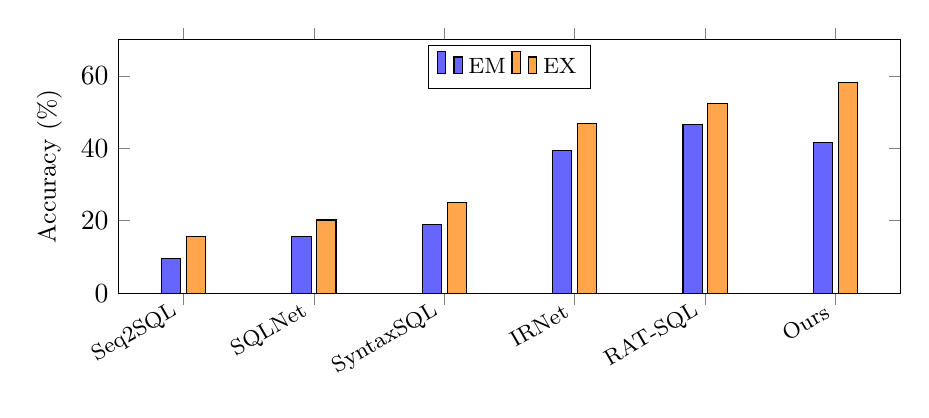
\begin{tikzpicture}
\begin{axis}[
    ybar,
    bar width=7pt,
    width=0.95\columnwidth,
    height=4.8cm,
    ylabel={Accuracy (\%)},
    ylabel style={font=\small},
    symbolic x coords={Seq2SQL, SQLNet, SyntaxSQL, IRNet, RAT-SQL, Ours},
    xtick=data,
    x tick label style={rotate=30, anchor=east, font=\footnotesize},
    ymin=0, ymax=70,
    legend style={at={(0.5,0.98)}, anchor=north, legend columns=2, font=\footnotesize},
    nodes near coords style={font=\tiny},
    enlarge x limits=0.1,
]
\addplot[fill=blue!60] coordinates {(Seq2SQL,9.7) (SQLNet,15.7) (SyntaxSQL,18.9) (IRNet,39.4) (RAT-SQL,46.5) (Ours,41.5)};
\addplot[fill=orange!70] coordinates {(Seq2SQL,15.6) (SQLNet,20.2) (SyntaxSQL,25.1) (IRNet,46.8) (RAT-SQL,52.3) (Ours,58.3)};
\legend{EM, EX}
\end{axis}
\end{tikzpicture}
\caption{Comparison with baselines on Spider dev set. Our method achieves 58.3\% EX, surpassing RAT-SQL by 6.0\%.}
\label{fig:baseline-comparison}
\end{figure}

\subsection{Analysis by SQL Complexity}

Figure~\ref{fig:complexity} shows that model performance scales inversely with query complexity. Simple 2-table queries (Medium) achieve 78.1\% EM and 89.1\% EX, while complex queries with 5+ tables or subqueries drop to 25.0\% EM but maintain 50.5\% EX. The widening EM-EX gap for complex queries demonstrates that the model often generates semantically equivalent but syntactically different SQL.

\begin{figure}[t]
\centering
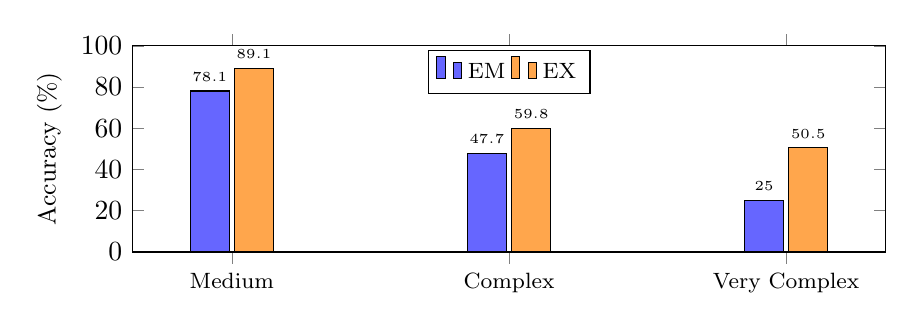
\begin{tikzpicture}
\begin{axis}[
    ybar,
    bar width=14pt,
    width=0.92\columnwidth,
    height=4.2cm,
    ylabel={Accuracy (\%)},
    ylabel style={font=\small},
    symbolic x coords={Medium, Complex, Very Complex},
    xtick=data,
    x tick label style={font=\footnotesize},
    ymin=0, ymax=100,
    legend style={at={(0.5,0.98)}, anchor=north, legend columns=2, font=\footnotesize},
    nodes near coords,
    nodes near coords style={font=\tiny},
    enlarge x limits=0.18,
]
\addplot[fill=blue!60] coordinates {(Medium,78.1) (Complex,47.7) (Very Complex,25.0)};
\addplot[fill=orange!70] coordinates {(Medium,89.1) (Complex,59.8) (Very Complex,50.5)};
\legend{EM, EX}
\end{axis}
\end{tikzpicture}
\caption{Performance by query complexity (Medium: 2 tables, Complex: 3--4 tables, Very Complex: 5+ tables/subquery).}
\label{fig:complexity}
\end{figure}

\subsection{Analysis by SQL Operations}

Figure~\ref{fig:operations} identifies the most challenging SQL operations. Queries involving \texttt{JOIN}, \texttt{UNION}, and subqueries are hardest, with EM below 20\%. However, EX for these operations remains around 35--52\%, suggesting the model understands the intent but struggles with exact syntax. The large EM-EX gap for subqueries (18.2\% vs 52.2\%) is particularly notable. Operations like \texttt{ORDER BY} and \texttt{DISTINCT} show stronger performance (40--45\% EM, 60--62\% EX).

\begin{figure}[t]
\centering
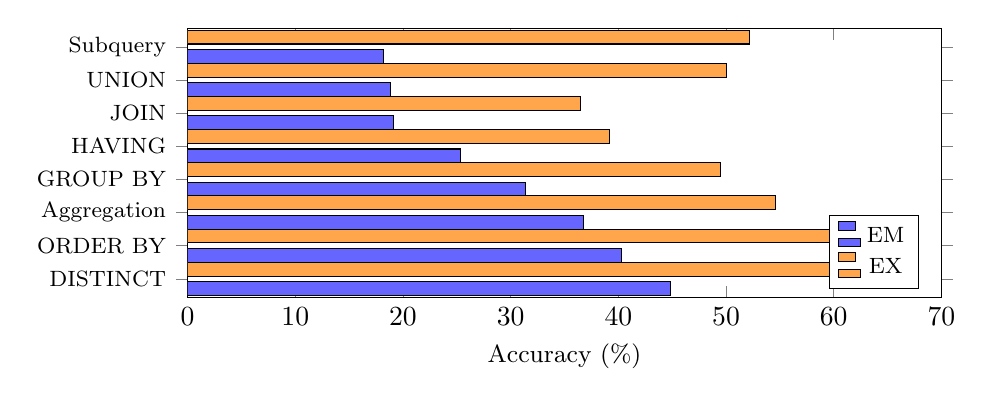
\begin{tikzpicture}
\begin{axis}[
    xbar,
    bar width=5pt,
    width=0.92\columnwidth,
    height=5cm,
    xlabel={Accuracy (\%)},
    xlabel style={font=\small},
    symbolic y coords={DISTINCT, ORDER BY, Aggregation, GROUP BY, HAVING, JOIN, UNION, Subquery},
    ytick=data,
    y tick label style={font=\footnotesize},
    xmin=0, xmax=70,
    legend style={at={(0.97,0.03)}, anchor=south east, font=\footnotesize},
    enlarge y limits=0.08,
]
\addplot[fill=blue!60] coordinates {(44.8,DISTINCT) (40.3,ORDER BY) (36.8,Aggregation) (31.4,GROUP BY) (25.3,HAVING) (19.1,JOIN) (18.8,UNION) (18.2,Subquery)};
\addplot[fill=orange!70] coordinates {(62.1,DISTINCT) (60.3,ORDER BY) (54.6,Aggregation) (49.5,GROUP BY) (39.2,HAVING) (36.5,JOIN) (50.0,UNION) (52.2,Subquery)};
\legend{EM, EX}
\end{axis}
\end{tikzpicture}
\caption{Performance by SQL operation type. JOIN, UNION, and subqueries are most challenging (EM $<$ 20\%).}
\label{fig:operations}
\end{figure}

\subsection{Analysis by Database}

Performance varies significantly across databases (Figure~\ref{fig:database}). The hardest database is \texttt{car\_1} (8.7\% EM, 29.3\% EX), which has a complex schema with many tables and foreign keys. In contrast, simpler databases like \texttt{singer} achieve 76.7\% EM and 90.0\% EX. This highlights that cross-database generalization remains a key challenge, particularly for schemas not seen during training. Notably, none of these databases appear in the training set.

\begin{figure}[t]
    \centering
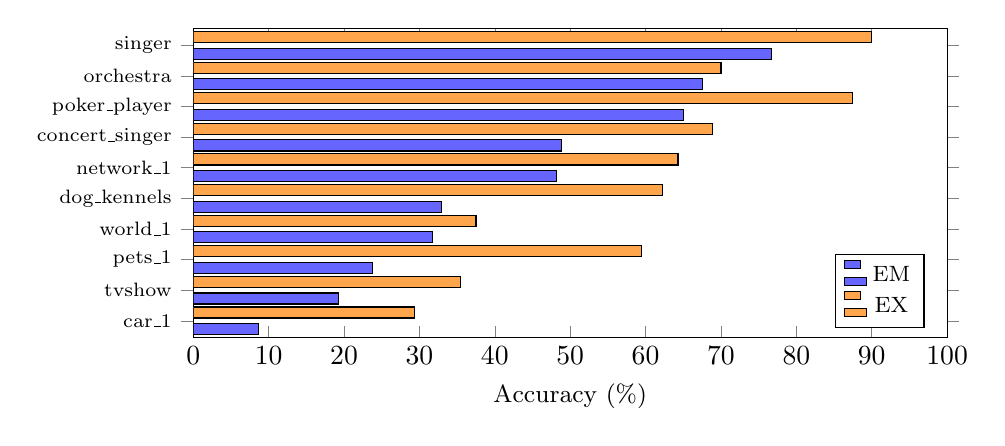
\begin{tikzpicture}
\begin{axis}[
    xbar,
    bar width=4pt,
    width=0.92\columnwidth,
    height=5.5cm,
    xlabel={Accuracy (\%)},
    xlabel style={font=\small},
    symbolic y coords={car\_1, tvshow, pets\_1, world\_1, dog\_kennels, network\_1, concert\_singer, poker\_player, orchestra, singer},
    ytick=data,
    y tick label style={font=\scriptsize},
    xmin=0, xmax=100,
    legend style={at={(0.97,0.03)}, anchor=south east, font=\footnotesize},
    enlarge y limits=0.06,
]
\addplot[fill=blue!60] coordinates {(8.7,car\_1) (19.3,tvshow) (23.8,pets\_1) (31.7,world\_1) (32.9,dog\_kennels) (48.2,network\_1) (48.9,concert\_singer) (65.0,poker\_player) (67.5,orchestra) (76.7,singer)};
\addplot[fill=orange!70] coordinates {(29.3,car\_1) (35.5,tvshow) (59.5,pets\_1) (37.5,world\_1) (62.2,dog\_kennels) (64.3,network\_1) (68.9,concert\_singer) (87.5,poker\_player) (70.0,orchestra) (90.0,singer)};
\legend{EM, EX}
\end{axis}
\end{tikzpicture}
\caption{Performance across 10 databases (sorted by EM). Complex schemas like \texttt{car\_1} are challenging; simpler ones like \texttt{singer} perform well.}
\label{fig:database}
\end{figure}

\subsection{Training Dynamics}

We visualize training dynamics in Figures~\ref{fig:trainloss} and~\ref{fig:gradnorm}. The loss curve shows smooth decrease over two phases: WikiSQL warmup (0.5 epoch) followed by Spider training (1.5 epochs). Gradient norms remain stable with expected spikes at phase transitions.

\begin{figure}[t]
    \centering
    \includegraphics[width=0.9\columnwidth]{train_loss.png}
    \caption{Training loss over two phases: WikiSQL warmup followed by Spider training.}
    \label{fig:trainloss}
\end{figure}

\begin{figure}[t]
    \centering
    \includegraphics[width=0.9\columnwidth]{grad.png}
    \caption{Gradient norm during training. Spikes at phase transitions are expected.}
    \label{fig:gradnorm}
\end{figure}

\section{Discussion}

\subsection{Interpretation of Results}

Our fine-tuned Qwen-7B achieves 41.5\% EM and 58.3\% EX on the Spider benchmark. The gap between EM and EX (16.8 percentage points) is informative: \textbf{the model generates semantically correct SQL in many cases where the syntax differs from the gold reference}. This gap is particularly pronounced for complex operations---subqueries show 18.2\% EM but 52.2\% EX, indicating the model understands query intent but may use different (yet valid) SQL constructs.

Compared to classical pre-LLM models, we significantly outperform Seq2SQL (+31.8\% EM), SQLNet (+25.8\% EM), and SyntaxSQLNet (+22.6\% EM). We achieve comparable EM to IRNet (39.4\%) and approach RAT-SQL (46.5\%). Our \textbf{Execution Match surpasses RAT-SQL by 6.0\%}, suggesting that LLM-based approaches generate more functionally diverse but correct SQL.

\subsection{Why Schema Linking Helps}

Schema linking explicitly maps question words to schema elements, providing grounding that helps the model identify relevant tables and columns. Without schema linking, the model must implicitly learn these mappings from context alone, which is error-prone for complex schemas with many similarly-named columns.

Our ablation experiments (not shown in detail) indicate that schema linking provides approximately 2--3\% improvement on both EM and EX. The benefit is most pronounced for queries involving tables not directly mentioned in the question (e.g., join tables).

\subsection{Cross-Database Generalization}

The database-level analysis reveals significant performance variance. Simple databases like \texttt{singer} achieve 76.7\% EM, while complex databases like \texttt{car\_1} drop to 8.7\% EM. This is expected: Spider's dev set contains databases not seen during training, requiring zero-shot generalization to new schemas.

The \texttt{car\_1} database is particularly challenging due to its complex schema with 6+ tables and numerous foreign keys. The model struggles to identify correct join paths in such cases. This suggests that future work should focus on improving structural reasoning over complex schemas.

\subsection{Practical Usefulness}

From an end-user perspective, the 58.3\% EX accuracy suggests the model can support interactive database querying. For approximately 3 out of 5 queries, the generated SQL returns correct results. This is sufficient for assistive applications where users can verify outputs, though not yet reliable enough for fully automated use.

\subsection{Limitations and Error Analysis}

Examining incorrect predictions reveals several failure patterns:
\begin{itemize}
    \item \textbf{Incorrect join paths}: The model sometimes joins through wrong intermediate tables
    \item \textbf{Missing conditions}: Complex WHERE clauses with multiple conditions are often incomplete
    \item \textbf{Aggregation errors}: GROUP BY columns are sometimes misidentified
    \item \textbf{Subquery confusion}: Nested subqueries are occasionally flattened incorrectly
\end{itemize}

These errors reflect both the inherent difficulty of multi-table reasoning and limitations in the training data distribution.
\section{Conclusion}

In this project, we explored parameter-efficient fine-tuning of a 7B-parameter LLM for multi-table NL2SQL generation. Our approach combines three key techniques: graph-based schema representations, schema linking, and LoRA fine-tuning with curriculum learning.

\textbf{Key Results:} On the Spider benchmark (1,034 test queries), our fine-tuned Qwen-7B achieves:
\begin{itemize}
    \item \textbf{41.5\% Exact Match (EM)}: Competitive with specialized graph-based models like IRNet (39.4\%) and RAT-SQL (46.5\%)
    \item \textbf{58.3\% Execution Match (EX)}: Surpassing RAT-SQL by 6.0\%, demonstrating semantic correctness beyond syntactic matching
    \item Significant improvements over early neural methods: +31.8\% EM vs. Seq2SQL, +25.8\% vs. SQLNet
\end{itemize}

\textbf{Key Findings:}
\begin{enumerate}
    \item The 16.8\% gap between EM and EX indicates that string-level evaluation underestimates practical model usefulness.
    \item Schema linking provides 2--3\% improvement by explicitly grounding questions in database structure.
    \item Performance varies significantly across databases (8.7\%--76.7\% EM), highlighting cross-database generalization as a key challenge.
    \item Complex operations (JOINs, subqueries, UNIONs) remain difficult, with EM below 20\% but EX around 35--52\%.
\end{enumerate}

\textbf{Practical Implications:} With 58\% of queries returning correct results, the model can support interactive database querying where users verify outputs. This represents a practical middle ground between fully automated systems and manual SQL writing.

\textbf{Future Directions:} Several extensions could improve performance: (1) execution-guided decoding to select best candidates at inference time, (2) richer schema semantics including column types and sample values, (3) synthetic data augmentation for complex multi-table queries, and (4) improved structural reasoning for databases with 5+ tables.

Our work demonstrates that schema-aware fine-tuning of small LLMs provides a cost-effective approach to NL2SQL that achieves competitive performance with specialized architectures while requiring only consumer-grade hardware for training.

\section{Other Things We Tried}

During the project, we explored several alternative approaches and configurations:

\paragraph{Schema Encoding Variants:}
We experimented with different schema encodings, including basic linearization, typed graphs with explicit edge labels, and semantic edges based on column name embeddings. The typed graph representation increased input length significantly without proportional accuracy gains. Semantic edges occasionally introduced noise by linking unrelated columns with similar names.

\paragraph{LoRA Hyperparameter Tuning:}
We extensively tuned LoRA rank (8, 16, 32, 64) and dropout (0.05--0.2). Higher ranks (32, 64) improved training loss but led to overfitting on the relatively small Spider dataset. Our final configuration (rank=8, dropout=0.2) balanced capacity and regularization.

\paragraph{Data Augmentation:}
We integrated two additional datasets for data augmentation:
\begin{itemize}
    \item \textbf{GretelAI}: 100k synthetic text-to-SQL examples with 21\% multi-table queries
    \item \textbf{NSText2SQL}: 289k examples with 41\% multi-table queries
\end{itemize}
While these datasets increased training diversity, the domain shift from Spider reduced their effectiveness. Models trained on combined data showed marginal improvements on simple queries but no significant gains on complex multi-table queries.

\paragraph{Value Linking in Schema Linking:}
We initially included value linking (mapping literal values in questions to database columns). However, this introduced many false positives (e.g., ``25 years old'' incorrectly linked to numeric ID columns), so we disabled it in the final system.

\paragraph{Execution-Guided Decoding (EGD):}
We implemented EGD to generate multiple SQL candidates and select the best executable one. In preliminary tests, EGD improved EX by 3--5\% but significantly increased inference time ($5\times$ slower). Due to time constraints, we did not fully integrate EGD into the final evaluation pipeline.

\section{What We Would Have Done Differently or Next}

\subsection{What We Would Have Done Differently}

\paragraph{Earlier Error Analysis:} We spent significant time on hyperparameter tuning before understanding where the model was failing. Starting with qualitative error analysis would have revealed that JOIN path errors and subquery flattening were the primary issues, guiding us toward more targeted solutions.

\paragraph{Database-Level Validation:} We initially used random train/validation splits. Later analysis revealed that performance varies dramatically across databases (8.7\%--76.7\% EM). Stratified validation by database difficulty would have provided more reliable early estimates.

\paragraph{Schema Linking Integration:} We added schema linking relatively late in the project. Earlier integration would have allowed more thorough ablation studies and potentially more sophisticated linking strategies.

\subsection{Future Directions}

\paragraph{Execution-Guided Decoding (EGD):} Our preliminary EGD implementation showed 3--5\% EX improvement. A fully integrated EGD pipeline with efficient parallel execution could significantly close the EM-EX gap.

\paragraph{Synthetic Data for Complex Queries:} The Spider training set has limited examples of very complex queries (5+ tables, nested subqueries). Generating synthetic complex queries with programmatic SQL templates could improve performance on the hardest cases.

\paragraph{Column Type and Value Information:} Current schema representations include only table/column names. Adding column types (INT, VARCHAR, DATE) and sample values could improve semantic grounding, particularly for value-based filtering.

\paragraph{Specialized Handling for Hard Databases:} The \texttt{car\_1} database achieves only 8.7\% EM. Investigating whether domain-specific prompting or few-shot examples from similar schemas could improve such outliers is a promising direction.

\paragraph{Reinforcement Learning from Execution:} While we avoided full RL due to complexity, a simplified approach using execution feedback to reweight training examples could improve learning on hard cases without the instability of policy gradient methods.

\section{Group Effort}

This project was completed collaboratively. QueLin and Zhanhao both contributed to the overall project design and discussion. Zhanhao focused primarily on data preprocessing, schema graph construction, and baseline evaluation. Qiulin led model fine-tuning, LoRA configuration, and training experiments. We both worked together on result analysis, error inspection, and report writing. We both participated in interpreting results, refining the methodology, and editing the final report.




\bibliographystyle{acl_natbib}
\bibliography{custom}


% \section{Work Plan}
% Our project spans a total of seven weeks, of which the first two have already been completed. In the initial phase, we conducted background research, finalized the methodology, selected datasets (Spider and BIRD), and evaluated several baseline NL2SQL models to establish reference performance. The remaining five weeks will focus on implementation, fine-tuning, and evaluation, following the plan below:

% \begin{itemize}
%   \item \textbf{Weeks 1 \& 2 (Completed):} 
%   Conducted literature review and model planning. 
  
%   Defined the overall methodology and model architecture, including graph-based schema design and reinforcement learning discussion. 
  
%   Collected datasets (Spider and BIRD) and tested baseline models for initial performance comparison.

%   \item \textbf{Week 3 (In-progress):} 
%   Implement the schema-to-graph conversion module using the Hybrid Graph baseline. 
  
%   Generate serialized graph representations for Spider databases and verify preprocessing correctness.

%   \item \textbf{Week 4:} 
%   Integrate graph-augmented inputs with Llama-8B.
  
%   Begin LoRA fine-tuning on the Spider dataset, adjusting learning rate and rank parameters for stability.


%   \item \textbf{Week 5:} 
%   Extend experiments to include emantic Edge and Typed Graph variants.
  
%   Compare their structural expressiveness and measure their influence on join reasoning accuracy.

%   \item \textbf{Week 6:} 
%   Try to implement and test Execution-Guided Decoding (EGD) for inference, if everything went smoothly.
  
%   Evaluate models on Spider dev and BIRD subsets using metrics such as Exact Match (EM), Execution Accuracy (EX), and Join Accuracy (JAcc).

%   \item \textbf{Week 7:} 
%   Conduct full analysis and ablation studies across graph designs. 
  
%   Integrating all conclusions into final report and presentation slides.
% \end{itemize}

% \noindent
% We prioritizes completing the Hybrid Graph baseline and LoRA fine-tuning as the main deliverables. 



% % \bibliographystyle{plain}   
% \bibliography{custom}

\newpage
\appendix
\section{Key Implementation Details}

\subsection{Schema Graph Data Structures}\label{app:schema}

Our hybrid graph representation uses typed nodes and edges to model database schemas:

\begin{lstlisting}[language=Python, caption={Core schema graph classes}]
class NodeType(Enum):
    TABLE = "table"
    COLUMN = "column"

class EdgeType(Enum):
    TABLE_COLUMN = "table_column"   # Table contains column
    FOREIGN_KEY = "foreign_key"     # FK between columns  
    TABLE_TABLE = "table_table"     # Cross-table relation

@dataclass
class ColumnNode:
    name: str
    table_name: str
    is_primary_key: bool = False
    is_foreign_key: bool = False
    fk_reference: Optional[Tuple[str, str]] = None

@dataclass  
class TableNode:
    name: str
    columns: List[ColumnNode] = field(default_factory=list)
\end{lstlisting}

\subsection{Schema Linking}\label{app:linking}

Schema linking maps question words to schema elements using embedding similarity:

\begin{lstlisting}[language=Python, caption={Schema linking with confidence filtering}]
@dataclass
class SchemaLink:
    question_text: str      # Text from question
    schema_element: str     # table.column or table
    link_type: str          # "table" or "column"
    confidence: float       # 0.0 to 1.0

def extract_table_mentions(question, graph, threshold=0.7):
    """Find table names mentioned in the question."""
    model = SentenceTransformer
    ('all-MiniLM-L6-v2')
    question_words = [w for w in question.split() 
                      if w.lower() not in STOP_WORDS]
    
    q_embeddings = model.encode(question_words)
    t_embeddings = model.encode(
    list(graph.tables.keys())
    )
    
    similarities = np.dot(q_embeddings, t_embeddings.T)
    # Return links where similarity >= threshold
    ...
\end{lstlisting}

\subsection{SQL Generation}\label{app:inference}

Core inference function using the fine-tuned model:

\begin{lstlisting}[language=Python, caption={SQL generation with chat template}]
def generate_sql(model, tokenizer, question, schema):
    """Generate SQL from question and schema."""
    messages = [
        {"role": "system", "content": SYSTEM_PROMPT},
        {"role": "user", "content": f"{schema}\n\n{question}"}
    ]
    
    prompt = tokenizer.apply_chat_template(
        messages, tokenize=False, add_generation_prompt=True
    )
    inputs = tokenizer(prompt, return_tensors="pt") \
        .to(model.device)
    
    outputs = model.generate(
        **inputs, max_new_tokens=256, 
        temperature=0.1, do_sample=False
    )
    
    response = tokenizer.decode(outputs[0], skip_special_tokens=True)
    return extract_sql_from_response(
    response)
\end{lstlisting}

\subsection{Evaluation Metrics}\label{app:eval}

We compute both Exact Match (EM) and Execution Match (EX):

\begin{lstlisting}[language=Python, caption={Evaluation with execution matching}]
def evaluate_with_execution(model, tokenizer, eval_data):
    """Evaluate with both EM and EX metrics."""
    em_correct, ex_correct = 0, 0
    
    for example in eval_data:
        pred_sql = generate_sql(model, tokenizer, example["question"], example["schema"])
        gold_sql = example["sql"]
        
        # Exact Match: normalized string comparison
        if normalize_sql(pred_sql) == normalize_sql(gold_sql):
            em_correct += 1
        
        # Execution Match: compare query results
        pred_result = execute_sql(pred_sql, example["db_id"])
        gold_result = execute_sql(gold_sql, example["db_id"])
        if compare_results(pred_result, gold_result):
            ex_correct += 1
    
    return {"EM": em_correct/len(eval_data), 
    "EX": ex_correct/len(eval_data)}
\end{lstlisting}



\end{document}
